\section{Experimental Evaluation}
\label{eval}


\subsection{Datasets and evaluation protocol} \label{eval:protocol}
We perform our experiments on three standard datasets for image retrieval: 
\begin{itemize}
    \item The INRIA \emph{Holidays} dataset \cite{holidays} which consists of 1491 images divided in 500 groups of matching images. We manually rotate by 90 degrees some images that are not in their natural orientation to compensate for the fact that CNN features are not rotation invariant~\cite{babenko14,Arandjelovic15,RaToCh16}.
    \item The \emph{Oxford5k} dataset \cite{oxford}, which consists of 5063 images separated in 55 groups of matching images, each group associated to a landmark of Oxford. We use the ``full'' crop, ignoring the region of interest of each image.
    \item The \emph{Oxford105k} dataset \cite{oxford}, a large-scale dataset containing the same images and queries from Oxford5k plus \emph{Flickr100k}, a collection of $10^5$ distractor Flickr images.
\end{itemize}
As pool of negative images to build SLEM, we use the Flickr100k for both Holidays and Oxford5k. When training on Oxford105k, we us instead the \emph{Paris} dataset \cite{PhiChIsSiZi08} as negative samples. \PP{Not clear: negatives are not all images from Flicker100k or Paris. $n$ random samples?}
%In both datasets, each group contains one query image, the other images in the group being the only correct answers to the query.
%For each query image, we calculate its similarity to all other images in the database and rank them in decreasing order.
%The average precision of a group is derived from the ranking of the images of the group for the similarity with the corresponding query image.
%The final mean average precision (mAP) for a dataset is the mean of the average precision over all its groups.
%As pool of negative images to build SLEM, we use the Flickr100k collection \cite{oxford}, composed of $10^5$ images from Flickr. For a full rank decomposition, we use only a subset of it, containing between 6000 and 15000 images.
%As stated in section \ref{low-rank} and further discussed in section \ref{time-scale}, a full rank decomposition does not scale well for bigger number of negative samples. For low rank decomposition, we use all 100000 images.

At evaluation time, for a dataset that consists of $p$ images and $q$ query images, we calculate the $p\times q$ \emph{similarity matrix} $S$, where each of its $q$ columns is the matching scores of the query image with all the $p$ images. \hlc{RR: maybe take out this paragraph completely.}

\begin{table*}[t!]
\begin{center}
\setlength{\tabcolsep}{.2em}
%\begin{tabular}{|c|c|c|c|c|c|c|c|}
%\small
\begin{tabular}{c@{\hskip 1em}cccc@{\hskip 1em}cccc@{\hskip 1em}cc}%@{\hskip 1em}c}
\toprule
Dataset & \multicolumn{4}{c}{\textbf{Holidays}} & \multicolumn{4}{c}{\textbf{Oxford 5k}} & \multicolumn{2}{c}{\textbf{Oxford 105k}} \\%& \textbf{Oxford 105k}\\
\midrule
Model, features & VLAD  & SPoC & AlexNet & NetVLAD & VLAD & SPoC & AlexNet & NetVLAD & SPoC & NetVLAD\\% & SPoC\\
\midrule
Baseline            & 72.7 & 76.5 & 68.2  &  85.4 & 46.3 & 54.4 & 40.6 & 67.5 & 50.1 & - \\% & \\
%Whitening           & -    & -    & -    & -    & -\\
PCAW                & 75.5 & 81.7 & 69.2 & 88.3 & 50.9  & 63.7 & 45.0 & 69.1 & 55.5 & - \\% & \\
LDA                 & 54.7 & 82.2 & 64.1 & 74.3 & 29.6  & 62.2 & 42.5 & 72.7 & 52.4 & - \\
ESVM~\cite{ZePe15}  & $77.5^3$ & $84.0^3$ & 71.3 & $91.4^2$ & 57.2  & 62.1 & 43.9 & 72.5 & 56.5 & - \\% & \\ 
Linear SLEM         & $78.0^2$ & 82.3 & 72.1 & $91.3^3$ & \ul{59.3}  & 64.1 & 46.2 & 72.9 & 56.7 & - \\% & \\ /42.2
Gaussian SLEM (16)  & 76.8 & 80.3 & 71.2 & $91.4^2$ & 52.8 & 63.0 & 43.5 & 71.9 & 55.8 & - \\
Gaussian SLEM (32)  & 77.4 & 81.7 & $72.0^3$ & $91.4^2$ & 54.9 & 63.1 & 44.0 & 71.1 & 56.0 & - \\
Gaussian SLEM (fr)  & \bf{78.1} & $86.2^2$ & \bf{72.9} & \bf{91.7} & 59.0   & \ul{64.9} & 47.0 & \ul{74.4} & 59.5 & - \\% & \\ 
Poly SLEM (16)      & 76.9 & 82.3 & 71.4 & $91.3^3$ & 53.0 & 63.6 & 43.6 & 71.4 & 56.1 & - \\
Poly SLEM (32)      & 77.3 & 82.4 & $72.1^2$ & \bf{91.7} & 54.9 & 63.6 & 44.1 & 71.6 & 56.3 & - \\
Poly SLEM   (fr)    & \bf{78.1} & \bf{86.3}  & \bf{72.9} & \bf{91.7} & \ul{59.3}  & 64.8 & \ul{47.3} & \ul{74.1} & 62.5 & - \\
\hline
\end{tabular}
\caption{Mean average precision results for INRIA Holidays and Oxford buildings datasets, expressed as percentages. In this table, we present our results for VLAD \cite{Delhumeau2013}, sum-pooling of convolutional features (SPoC) \cite{babenko15}, activation coefficients from the previous-to-last CNN layer (AlexNet) \cite{Krizhevsky2012} and activation of NetVLAD layer~\cite{Arandjelovic15}. In parenthesis, the rank of he decomposition (`fr' for full rank decomposition) \PP{meaning of bold and underline}}
\label{fullrank}
\end{center}
\end{table*}

\subsection{Which kernel to choose?}
For the experiment of SLEM as a feature encoder, we tested two different kernels -- Gaussian and polynomial -- each with a scalar parameter $\gamma$:
\begin{align}
    k_1(x,y) = e^{-\gamma\|x-y \|^2}; \ 
    k_2(x,y) = x^Ty+\gamma(x^Ty)^2. \label{kernels}
\end{align}
\textbf{Gaussian SLEM.} The radial basis function kernel $k_1$ is a
well known reproducing kernel, used for classification with support vector machines.\\
\textbf{Poly SLEM.} The polynomial kernel $k_2$ is a reproducing kernel often used in natural language processing.\\
%Note the non-kernel version of SLEM is equivalent to a SLEM for the linear kernel. In order to distinguish it from other versions, we will refer to the non-kernel version as \textbf{Linear SLEM} for the remaining of this paper.
%\textbf{SPM SLEM} The spatial pyramid matching kernel of $L+1$ levels in Equation \ref{k:spm} take as input a set of local descriptors and its location in pyramidal bins \cite{spk}. 


\subsection{Base visual features}
We test our feature encoder for four different base features: the hand-crafted VLAD image representation and three learned features derived from the activation coefficients of deep Convolutional Neural Networks.

We use the same VLAD variant of \cite{Delhumeau2013} used in \cite{ZePe15} that relies on densely-extracted rootSIFT \cite{3things} local descriptors, per-cluster normalization, PCA-based rotations, and root normalization. Like \cite{ZePe15}, we use $64$ clusters, for a final feature of size $8192$.

The first CNN-based features we use consist of the activation coefficients of the previous-to-last layer of the AlexNet architecture \cite{Krizhevsky2012}, based on a publicly available pre-trained model \cite{jia2014caffe}. These are also the features used in \cite{ZePe15}.

The SPoC features \cite{babenko15}, which are tailored specifically for the image retrieval application, consist of spatially-weighted sums of the activations of the last convolutional layer of a 19-layer CNN \cite{SimonZisser15}.

Finally, we use the NetVLAD features \cite{Arandjelovic15}, trained for place recognition. These features are obtained by adding a differentiable version of the VLAD algorithm~\cite{Delhumeau2013} as a layer at the end of a convolutional architecture.


%We revisit the VLAD feature presented in \cite{VLAD} as an example of a hand-crafted representation. First we extract a set $\mathcal{F}$ of local descriptors of the image $I$. We use the 128 dimension RootSIFT \cite{3things} descriptors, extracted densely.
%Then, we hard-assign each descriptor $f$ in $\mathcal{F}$ to the closest among $K$ pre-trained codewords $c_k$, $k\in\{1\cdots K\}$,
%one of $K$ set $\mathcal{C}_k$ of descriptors associated to codewords $\{c_k\}_{1\leq k\leq K}$, 
%and map $f$ to a $\RR^{128K}$ vector
%\begin{equation}
%\phi^{VL}_1(f) = \left[0 \cdots 0\quad \Phi_k^T\frac{(f-c_k)}{\|f-c_k\|} \quad 0 \cdots 0\right],
%\end{equation}
%where $\Phi_k$ is a $128\times 128$ PCA matrix learned on training features mapped to $k$-the codeword.
%associated to descriptors in $\mathcal{C}_k$. 
%The final VLAD representation is the power-normalization and $l_2$ normalization of the sum-pooling of $\phi^{VL}_1$:
%\begin{equation}
%\phi^{VL}_2(I) \propto \mathrm{power}\big(\sum_{f\in \mathcal{F}}\phi^{VL}_1(f)\big),~\|\phi^{VL}_2(I)\|=1,
%\end{equation}
%with scalar power normalization $\mathrm{power}(v)=\mathrm{sign}(v)|v|^{0.2}$ applied component-wise.
%In experiments, we use $K=64$ codewords learned on images from Flickr. Our VLAD representation has $d=8192$ dimensions.

%Convolutional features obtained from very deep convolutional neural networks (CNNs) have been shown to work as good local descriptors for matching \cite{SimonZisser15}. The SPoC representation \cite{babenko15} is a weighted sum-pooling of the activations of the last convolutional layer of a 19-layer CNN. For a given input image $I$, the activations in this layer are organized over a $W\times H$ spatial grid and over $d$ channels. Each position $(w,h)$ in $\{1 \cdots W\}\times \{1\cdots H\}$ can thus be equipped with a descriptor $f_{h,w}(I)$ in $\RR^D$.
%Indeed, if our last convolutional layer has $D$ neurons, and each neuron a $W\times H$ map of activations of this neurons to the image $I$, 
%each pair $(w,h)$ with $w$ in $\{1,2,..., W\}$ and $h$ in $\{1,2,...,H\}$ can be associated to a descriptor $f_{(h,w)}$ in $\RR^D$ of the responses of each neuron at coordinate $(w,h)$ of the maps. 
%We then sum-pool these descriptors, weighted accordingly to their distance to the center of the image:
%\begin{equation}
%    \phi^{SPoC}(I) = \sum_{w=1}^W\sum_{h=1}^H \alpha_{w,h}f_{w,h}(I),
%\end{equation}
%where
%\begin{equation}
%    \alpha_{w,h} = \exp \left(-\dfrac{(w-W/2)^2+(h-H/2)^2}{2\sigma^2}\right).
%\end{equation}
%In our experiments, we follow the implementation details of \cite{babenko15}: We resize all images to $586\times 586$ pixels before feeding them to the network. The last convolutional layer has $d=512$ channels with activation maps of size $(W,H)=(37,37)$, and we set $\sigma=\frac{H}{3}$. We use the same network architecture to extract the convolutional maps but different weights in the convolutional layer, which might explain the difference between the results in Table \ref{fullrank:results} and \cite{babenko15}.

%Finally, we also test a more convencional CNN feature, less deep and using two fully connected layers after the convolutional layers.
%Our final representation is a $4096$ non-negative feature. We based out implementation on CAFFE \cite{jia2014caffe}.



\subsection{Image retrieval results}
We use the base features of the previous subsection as baseline. Since Babenko \etal~\cite{babenko15} and Arandjelovi\'c \etal~\cite{Arandjelovic15} have improved retrieval results by applying PCA followed by whitening to their features, we also apply this post-processing to our base features as second baseline (PCAW), compressing base feature dimension to half of the original. We then compare the baselines with the original ESVM, LDA and several variants of our approach (SLEM), since all the those methods are based on similar \hlc{??? (I can't read the last word you wrote.} The results are presented in Table \ref{fullrank}. \PP{Explain why fewer columns for Oxford105k}

Linear SLEM performs similarly to ESVM despite being much more time efficient (see discussion in Section \ref{time-scale}). 
The fact that a hinge loss classifier does not outperform a square loss classifier can seem counter-intuitive, but both were shown to be equivalent for binary classification under mild constraints~\cite{YeXi07}.

We perform both Gaussian SLEM and Polynomial SLEM with two decompositions: one full-rank CCD decomposition signaled by ``(fr)'' and two low-rank KPCA decompositions signaled by the rank of the decomposition. We train our exemplar classifiers for between $6000$ and $15000$ negative samplers. For all the experiments we calibrate the regularization cost $\lambda$, as well as the parameter $\gamma$. 

The full-rank variant outperforms all methods for all base features, although the gains when compared to linear SLEM are not always significant (\emph{e.g.} for VLAD features). It is interesting to notice that LDA, ESVM and Linear SLEM do not seem to outperform one another or the baselines consistently for all features and datasets.
%For VLAD and AlexNet, we considere the version presented in~\cite{ZePe15} as \textit{Baseline} and a rotated, whitened and compressed to half its original dimensions as \textit{PCA+whitening}. 
%As for the version of each feature to which we apply the other algorithms, it changes according to the dataset. 
%For SPoC, we apply LDA, ESVM and SLEM to the baseline, as a replacement of PCA. 
%For NetVLAD, we use the rotated and compressed version of the trained networks correspondent to each dataset as suggested by~\cite{Arandjelovic15}. 
%For Holidays we obtain better results with whitened features and for Oxford5k, non-whitened.

%For \textit{LDA}, we follow our description in section \ref{sec:lda} and calculate $\Sigma$ as the convariance of the negative samples.
%In our experiments, the compression worsens the results when compared with non-compressed. \textit{Delhumeau et al.}~\cite{Delhumeau2013}
%Hence we compare the improvements of PCA plus whitening, without compression, with our method.



%For some experiments, specially using VLAD, the optimal value of $\gamma$ is rather small ($\gamma\sim 0.05$), which suggests the linear kernel is already close to the optimal kernel for these features.

\begin{figure*}
  \begin{tikzpicture}
    \begin{groupplot}
      [group style={%
        columns=2,
        rows=1,
        group name=plots,
        xlabels at=edge bottom,
        %y descriptions at=all,
        horizontal sep=5em,        
      },
      % ybar,
      % ymin=0,
      % ymax=27e3,
      enlarge x limits={abs=.5},
      width=0.5\textwidth,
      height=0.4\textwidth,
      % scaled y ticks=base 10:-3,
      % xticklabels from table={\first}{Criterion},
      % x tick label style={rotate=90,anchor=east},
      % xtick=data,
      ]

      \nextgroupplot[xlabel=Num. $n$ of negatives,
      ylabel=mAP]
      ]
      %% Poly SLEM
      \addplot[PolySLEM] coordinates {%gamma=10^-3, lambda=10^-3
        (500,  0.81905)
        (1500, 0.83777)
        (2500, 0.83924)
        (3500, 0.84502)
        (4500, 0.85089)
        (5500, 0.85432)
        (6500, 0.85364)
        (7500, 0.85724)
        (8500, 0.85571)
        (9500, 0.86146)
        (10500,0.86133)
        (11500,0.86163)
        (12500,0.86186)
        (13500,0.86122)
        (14500,0.86336)
      };
      %% Gaussian SLEM
      \addplot[GaussSLEM] coordinates {
        (500,  0.82525)
        (1500, 0.83943)
        (2500, 0.84025)
        (3500, 0.84782)
        (4500, 0.85128)
        (5500, 0.85385)
        (6500, 0.85434)
        (7500, 0.85740)
        (8500, 0.85364)
        (9500, 0.85806)
        (10500,0.86022)
        (11500,0.86172)
        (12500,0.85862)
        (13500,0.86062)
        (14500,0.86180)
      };
      %% ESVM8
      \addplot[ESVM] coordinates {
        (500,  0.81446)
        (1500, 0.82524)
        (2500, 0.82707)
        (3500, 0.82359)
        (4500, 0.82719)
        (5500, 0.82689)
        (6500, 0.82993)
        (7500, 0.83019)
        (8500, 0.82972)
        (9500, 0.83280)
        (10500,0.83289)
        (11500,0.83457)
        (12500,0.83421)
        (13500,0.83968)
        (14500,0.83995)
      };
      %% Linear SLEM
      \addplot[LinSLEM] coordinates {%lambda = 10^-3
        (500,  0.81524)
        (1500, 0.81843)
        (2500, 0.82042)
        (3500, 0.81973)
        (4500, 0.81862)
        (5500, 0.81760)
        (6500, 0.82291)
        (7500, 0.82330)
        (8500, 0.82092)
        (9500, 0.82221)
        (10500,0.81929)
        (11500,0.82335)
        (12500,0.82301)
        (13500,0.82254)
        (14500,0.82311)
      };

      \nextgroupplot[
      ymode=log,
      xlabel=Num. $n$ of negatives,
      ylabel=Time per image (s),
      legend to name=grouplegend,
      legend style={legend columns=-1},
      % legend style={at={(0.465,-0.45)},
      % anchor=north,legend columns=-1},
      ]%
      %% Poly SLEM
      \addplot[PolySLEM] coordinates {
        (500,  0.0002099)
        (1500, 0.0009621)
        (2500, 0.0026628)
        (3500, 0.0054810)
        (4500, 0.0086532)
        (5500, 0.0121226)
        (6500, 0.0188800)
        (7500, 0.0228739)
        (8500, 0.0434941)
        (9500, 0.0499160)
        (10500,0.0477895)
        (11500,0.0703987)
        (12500,0.0842496)
        (13500,0.0802379)
        (14500,0.1245190)
      };
      \addlegendentry{Poly SLEM}
      %% Gaussian SLEM
      \addplot[GaussSLEM] coordinates {
        (500,  0.0006671)
        (1500, 0.0012690)
        (2500, 0.0027834)
        (3500, 0.0055151)
        (4500, 0.0094601)
        (5500, 0.0140014)
        (6500, 0.0184553)
        (7500, 0.0249103)
        (8500, 0.0430012)
        (9500, 0.0539018)
        (10500,0.0617439)
        (11500,0.0695579)
        (12500,0.0865806)
        (13500,0.1049192)
        (14500,0.1037325)
      };
      \addlegendentry{Gaussian SLEM}
      %% ESVM
      \addplot[ESVM] coordinates {
        % (600, .000610)
        % (6000, .00427)
        % (60000, .0378)
         (1000 * 6/10, .000610)%(1000 * 6/10, .002440)
        (10000* 6/10, .00427)%(10000* 6/10, .01708)
        (14500, .0095478)%(14500, .0382) %Interpolated
        % (100000 * 6/10, .0378)
        % (500,  0.014)
        % (1500, 0.015)
        % (2500, 0.016)
        % (3500, 0.017)
        % (4500, 0.018)
        % (5500, 0.019)
        % (6500, 0.02)
        % (7500, 0.021)
        % (8500, 0.022)
        % (9500, 0.023)
        % (10500,0.024)
        % (11500,0.025)
        % (12500,0.026)
        % (13500,0.027)
        % (14500,0.028)
      };
      \addlegendentry{ESVM}
      %% Linear SLEM
      \addplot[LinSLEM] coordinates {
        (500,  0.0000622)
        (1500, 0.0000704)
        (2500, 0.0000581)
        (3500, 0.0000592)
        (4500, 0.0000902)
        (5500, 0.0000655)
        (6500, 0.0001069)
        (7500, 0.0000973)
        (8500, 0.0000914)
        (9500, 0.0000812)
        (10500,0.0000923)
        (11500,0.0001047)
        (12500,0.0001122)
        (13500,0.0001251)
        (14500,0.0001156)
      };
      \addlegendentry{Linear SLEM}
      \addplot[mark=*, green, dashed] coordinates {
            (500,  0.0001208)
            (1500, 0.0003114)
            (2500, 0.0008255)
            (3500, 0.0016757)
            (4500, 0.0017118)
            (5500, 0.0025198)
            (6500, 0.0033489)
            (7500, 0.0042703)
            (8500, 0.0060299)
            (9500, 0.0074267)
            (10500,0.0094138)
            (11500,0.0113405)
            (12500,0.0121783)
            (13500,0.0144320)
            (14500,0.0171987)
          };
      \addplot[mark=*, blue, dashed] coordinates {
            (500,  0.0001501)
            (1500, 0.0003122)
            (2500, 0.0006261)
            (3500, 0.0011822)
            (4500, 0.0015350)
            (5500, 0.0023396)
            (6500, 0.0047356)
            (7500, 0.0051036)
            (8500, 0.0061753)
            (9500, 0.0092072)
            (10500,0.0101006)
            (11500,0.0117932)
            (12500,0.0154758)
            (13500,0.0185985)
            (14500,0.0194114)
          };
      
      


    \end{groupplot}

    \node at (plots c1r1.north east) [anchor=south, xshift=2.5em] {\ref{grouplegend}};
    %\draw (plots c2r1.north west) circle (3pt) node {North west};

  \end{tikzpicture}
  \caption{Results for INRIA Holidays, using SPoC features and different methods of SLEM (see legend). We use $T=10^5$ iterations for all $n$ to report mAP for ESVM, as suggested by \cite{ZePe15}, but report timings using $T=1.66 n$ and the values reported in Table 1 of \cite{ZePe15}. Left: mAP; Right: computation time in solid line, \emph{online} computational cost in dashed line.}
  \label{fullrank:results}
\end{figure*}



\subsection{Time and storage scalability} \label{time-scale}
In this section we compare the time efficiency of our method and the ESVM, as well as discuss which method and decomposition to use accordingly with the number of positive and negative samples.

In Fig. \ref{fullrank:results}, we see that the Linear SLEM efficiency does not change with $n$.
Indeed, if $d$ is the dimension of the base representation, $A$ is a $d\times d$ matrix for linear SLEM, whereas for a full rank kernel, $A$ is $n\times n$.
This explains the increasing running time for Gaussian and polynomial kernels: storage and solving a $n\times n$ system does not scale for large number of negative samples.

Retrieval results for full-rank kernelized SLEM in Fig. \ref{fullrank:results} suggest we can benefit from larger sets of negative samples. We however limit our full-rank experiments to 15000 negatives samples due to the $O(n^3)$ complexity of the offline step.
When we consider only the online procedure of our model, \emph{i.e.} the calculation of $\beta^\star$, our kernelized model has a similar time-efficiency to ESVM. Therefore, we can process the kernel SLEM for the Gaussian and polynomial kernels with similar running time to ESVM if we pre-process our negative samples offline.

For the low-rank decomposition, we present in Fig. \ref{kpca:icd} a comparison in average precision between KPCA and ICD decompositions using SPoC on the Holidays dataset. The superior results justify our preference for KPCA, despite its time-inefficient offline step. The only advantage of ICD over KPCA is its time complexity, linear in the number of negative samples, that allows a bigger number of negative samples. In Fig. \ref{icd} we show results of ICD for bigger pools of negative samples. The results suggest that performance of low-rank SLEM is not sensible to the number of negative samples.

\begin{figure}[!h]
\centering
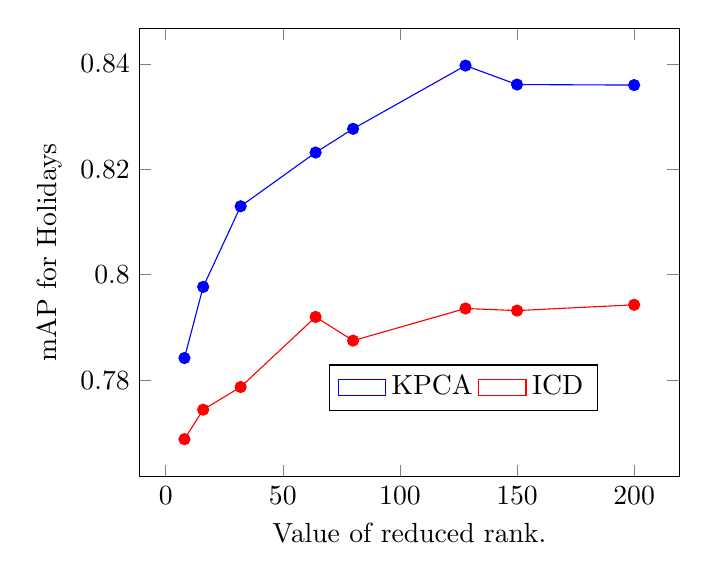
\begin{tikzpicture}
	\begin{axis}[
		xlabel=Value of reduced rank.,
		ylabel=mAP for Holidays,
		legend style={
			area legend,
			at={(0.6,0.25)},
			anchor=north,
			legend columns=-1}]
%%Poly SLEM
    \addplot[mark=*, blue] coordinates{
        (  8, 0.7842)
        ( 16, 0.7977)
        ( 32, 0.8130)
        ( 64, 0.8232)
        ( 80, 0.8277)
        (128, 0.8397)
        (150, 0.8361)
       ( 200, 0.8360)
    };
    \addlegendentry{KPCA}
    \addplot[mark=*, red] coordinates{
        (  8, 0.7688)
        ( 16, 0.7744)
        ( 32, 0.7787)
        ( 64, 0.7920)
        ( 80, 0.7875)
        (128, 0.7936)
        (150, 0.7932)
       ( 200, 0.7943)
    };
    \addlegendentry{ICD}
	\end{axis}
\end{tikzpicture}
\caption{mAP for Holidays using SPoC + Poly SLEM. We perform two low-rank decompositions and compare its results at similar ranks.}
\label{kpca:icd}
\end{figure}



\begin{figure}[!h]
\centering
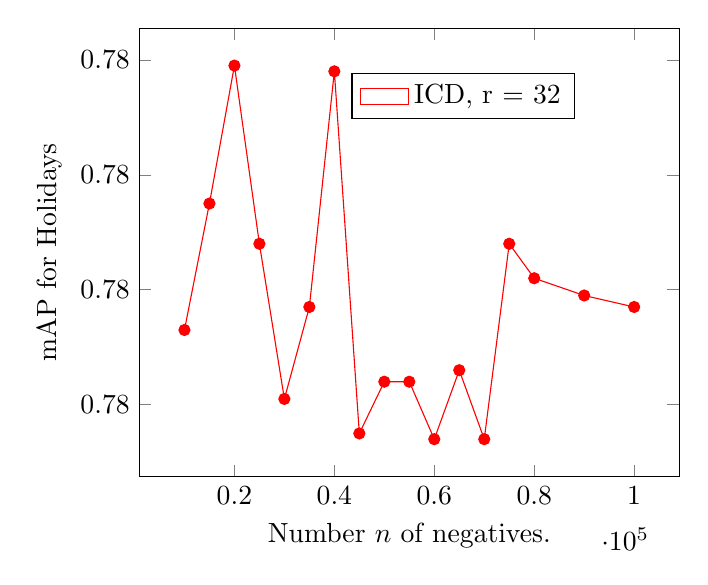
\begin{tikzpicture}
	\begin{axis}[
		xlabel=Number $n$ of negatives.,
		ylabel=mAP for Holidays,
		legend style={
			area legend,
			at={(0.6,0.9)},
			anchor=north,
			legend columns=-1}]
%%Poly SLEM
    \addplot[mark=*, red] coordinates{
        (  10000, 0.7773)
        (  15000, 0.7795)
        (  20000, 0.7819)
        (  25000, 0.7788)
        (  30000, 0.7761)
        (  35000, 0.7777)
        (  40000, 0.7818)
        (  45000, 0.7755)
        (  50000, 0.7764)
        (  55000, 0.7764)
        (  60000, 0.7754)
        (  65000, 0.7766)
        (  70000, 0.7754)
        (  75000, 0.7788)
        (  80000, 0.7782)
       (   90000, 0.7779)
       (  100000, 0.7777)
    };
    \addlegendentry{ICD, r = 32}
	\end{axis}
\end{tikzpicture}
\caption{mAP for Holidays using SPoC + Poly SLEM, using ICD and fixed 32-rank.}
\label{icd}
\end{figure}


\vspace{3 mm}



\subsection{Comparation to the state of the art}
We compare our results to the state of the art for Holidays and Oxford 5k in Table ~\ref{sota}.  We do not include re-ranking nor query expansion. We compare the state of the art global descriptors to both SPoC and NetVLAD features improved by Linear SLEM and low-rank Poly SLEM for rank equals to 16 and 32. We perform PCA and whitening to reduce the dimension of both descriptors to 256 and 512, and compare results by bracket of dimension. We also add a bracket of the full 4096-dimension NetVLAD for completeness, so we include our best performance. Our approach outperforms the state of the art for Holidays, despite not using descriptors as base feature. \PP{A word on Ox5k, where we are far behind Gordo? Something special about this dataset?}

\begin{table}[t]
\begin{center}
\setlength{\tabcolsep}{.2em}
\small
\begin{tabular}{l|c|ll}
\toprule
Features & dim & \textbf{Hol.} & \textbf{Ox5k} \\%& \textbf{Oxford 105k}\\
\midrule
Babenko \textit{et al.}\cite{babenko15}  & 256 & 80.2 & 58.9 \\ %& 57.8\\
Radenovi\'c \textit{et al.} \cite{RaToCh16}   & 256 & 81.5 & \un{77.4} \\
Arandjelovi\'c \textit{et al.} \cite{Arandjelovic15}& 256 & 86.0 & 62.5 \\ %& - \\
Kalantidis  \textit{et al.} \cite{KaMeOs16}   & 256 & 83.1 & 65.4 \\
SPoC + Linear SLEM & 256 & 81.5 & 64.7 \\
SPoC + Poly SLEM & 288 & 80.1 & 63.6 \\
SPoC + Poly SLEM & 320 & 81.8 & 63.6 \\
NetVLAD + Linear SLEM & 256 & \un{88.5} & 65.9 \\
NetVLAD + Poly SLEM & 288 & 87.7 & 65.5 \\
NetVLAD + Poly SLEM & 320 & 88.3 & 65.6 \\
\midrule
Radenovi\'c \textit{et al.} \cite{RaToCh16}   & 512 & 82.5 & 79.7 \\
Arandjelovi\'c \textit{et al.} \cite{Arandjelovic15}& 512 & 86.7 & 65.6 \\
Kalantidis \textit{et al.} \cite{KaMeOs16}   & 512 & 84.9 & 68.2 \\
Gordo \textit{et al.} \cite{GoAlReLa16} & 512 & 89.1^{\dag} & \bf{83.1}^{\dag} \\
SPoC + Linear SLEM & 512 & 82.3 & 64.1 \\
SPoC + Poly SLEM & 544 & 82.3 & 63.0 \\
SPoC + Poly SLEM & 576 & 82.4 & 63.1 \\
NetVLAD + Linear SLEM & 512 & 89.3 & 72.3 \\
NetVLAD + Poly SLEM & 544 & \un{89.9} & 71.9 \\
NetVLAD + Poly SLEM & 576 & \un{89.9} & 72.3 \\
\midrule
Arandjelovi\'c \textit{et al.} \cite{Arandjelovic15}& 4096 & 88.3 & 69.1 \\
%Li \textit{et al.} \cite{LiLaHa15}& - & 89.2^{\dag} & 73.7 \\
NetVLAD + Linear SLEM & 4096 & 91.3 & 72.9 \\
NetVLAD + Poly SLEM & 4128 & 91.3 & 71.2 \\
NetVLAD + Poly SLEM & 4160 & \bf{91.7} & 71.7 \\
%Zepeda \textit{et al.} \cite{ZePe15} & \underline{78.3} & - & 71.8 & - & 57.5 & - & 44.6 & - & - \\
%Babenko \textit{et al.} \cite{babenko15} & - & 81.8 & - & - & - & \textbf{65.7} & - & - & 57.8\\
\hline 
\end{tabular}
\caption{Compared results to state-of-the-art features at similar dimensions, without re-ranking or query augmentation. The results using Poly SLEM or Gaussian SLEM add 32 or 64 dimensions to the original feature (for $r=16$ or $r=32$, respectively). Underlined results are the best at each dimension bracket and bold results are the general best. $\dag$ indicates the previous state-of-the-art.}
\label{sota}
\end{center}
\end{table}

%\subsection{Semantic correspondence results}

%\subsection{Classification results}
